% Chapter 4 (from main tex file)
% Research Project
% Author: Javier Reyes

\chapter{Software Application} \label{software-application}

The current application is in WIP (Work In Progress) state, as there are technical challenges to
overcome. Esentially, the application is coded in C (with an option created in C++ for testing), and
built in the Xilinx SDK via the cross-compilers that Xilinx provide for the ARM7 architecture.

\section{Architecture}

The program follows a simple principle, with a single thread execution, but can be expanded with a
thread definition for the handling of the hardware control.

\begin{figure}[htp]
	\centering
	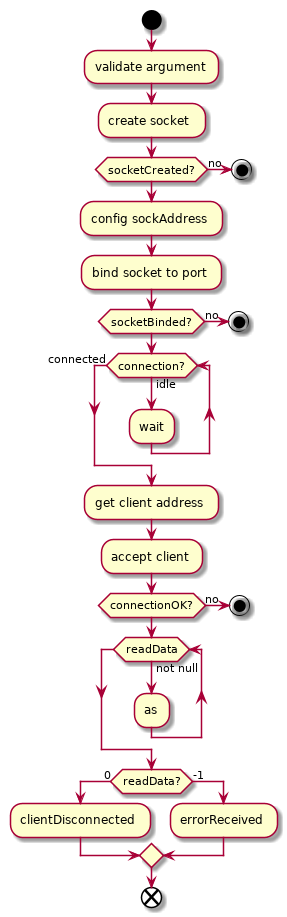
\includegraphics[width=0.7\textwidth]{activity-diag-eth.png}
	\caption{Activity diagram for server application in Zynqberry.}
	\label{fig:activity-diag-eth}
\end{figure}

Given the expected workflow for developing Linux applications for a Zynq device, the application
should be included in the image building process (with the
\texttt{petalinux-create -t apps --name myApp}), so that it can be installed properly in the system.
The previous workflow expects an INITRAMFS, which is not the case we used. Therefore, we had to
manually copy the application executable into the rootfs of the Zynqberry. The simplest way is to
use \texttt{scp} command with the Zynqberry connected to the local network.

As mentioned in chapter \ref{chapter1}, the Zynqberry device should be able to receive a video
stream from the Cam Controller device. Is it then necessary that the application acted as a server,
for the client application that was developed for the Cam Controller device, and described in
\cite{Poliakov2018}.

In order to handle a hardware processing functionality in the PL part of the Zynq device, a driver
module needs to be included, which provides the methods for read/write operations to the memory
block that is mapped to the IP Core. This part is not shown in the diagram, as it is neither
functional nor validated.

\section{Memory maped FPGA registers}

This section presents the expected design to be programmed into the PL part of the Zynq. It should
be noted that the design is not yet validated, and is on test phase, as has proven to be difficult
to make a DMA module to work.

The estandar way to work with the PL is described in UGXXX. The logic is expressed with the use of
predefined IP cores as blocks.

\section{CAN Communication}

As the communication with the rest of the devices is performed via CAN, the image was built with the
CAN module kernel enabled. The usage of the CAN device is still in debug state, as the recommended
flow is to use the CANutils device drivers, available from the apt repositories for the Xilinx
Linux, but this has not worked as expected. It should be noted that the Standalone usage of the CAN
module in the Zynqberry works flawlessly, and that the material presented by Xilinx related to
the usage of CAN in the Linux image is contradictory to the configuration present in the petalinux
template provided by the manufacturer.

% TODO: Complete chapter
